\documentclass[12pt,a4paper,]{book}
\def\ifdoblecara{} %% set to true
\def\ifprincipal{} %% set to true
\let\ifprincipal\undefined %% set to false
\def\ifcitapandoc{} %% set to true
\let\ifcitapandoc\undefined %% set to false
\usepackage{lmodern}
% sin fontmathfamily
\usepackage{amssymb,amsmath}
\usepackage{ifxetex,ifluatex}
%\usepackage{fixltx2e} % provides \textsubscript %PLLC
\ifnum 0\ifxetex 1\fi\ifluatex 1\fi=0 % if pdftex
  \usepackage[T1]{fontenc}
  \usepackage[utf8]{inputenc}
\else % if luatex or xelatex
  \ifxetex
    \usepackage{mathspec}
  \else
    \usepackage{fontspec}
  \fi
  \defaultfontfeatures{Ligatures=TeX,Scale=MatchLowercase}
\fi
% use upquote if available, for straight quotes in verbatim environments
\IfFileExists{upquote.sty}{\usepackage{upquote}}{}
% use microtype if available
\IfFileExists{microtype.sty}{%
\usepackage{microtype}
\UseMicrotypeSet[protrusion]{basicmath} % disable protrusion for tt fonts
}{}
\usepackage[margin = 2.5cm]{geometry}
\usepackage{hyperref}
\hypersetup{unicode=true,
            pdfauthor={Nombre Completo Autor},
              pdfborder={0 0 0},
              breaklinks=true}
\urlstyle{same}  % don't use monospace font for urls
%
\usepackage[usenames,dvipsnames]{xcolor}  %new PLLC
\IfFileExists{parskip.sty}{%
\usepackage{parskip}
}{% else
\setlength{\parindent}{0pt}
\setlength{\parskip}{6pt plus 2pt minus 1pt}
}
\setlength{\emergencystretch}{3em}  % prevent overfull lines
\providecommand{\tightlist}{%
  \setlength{\itemsep}{0pt}\setlength{\parskip}{0pt}}
\setcounter{secnumdepth}{5}
% Redefines (sub)paragraphs to behave more like sections
\ifx\paragraph\undefined\else
\let\oldparagraph\paragraph
\renewcommand{\paragraph}[1]{\oldparagraph{#1}\mbox{}}
\fi
\ifx\subparagraph\undefined\else
\let\oldsubparagraph\subparagraph
\renewcommand{\subparagraph}[1]{\oldsubparagraph{#1}\mbox{}}
\fi

%%% Use protect on footnotes to avoid problems with footnotes in titles
\let\rmarkdownfootnote\footnote%
\def\footnote{\protect\rmarkdownfootnote}


  \title{}
    \author{Nombre Completo Autor}
      \date{18/11/2021}


%%%%%%% inicio: latex_preambulo.tex PLLC


%% UTILIZA CODIFICACIÓN UTF-8
%% MODIFICARLO CONVENIENTEMENTE PARA USARLO CON OTRAS CODIFICACIONES


%\usepackage[spanish,es-nodecimaldot,es-noshorthands]{babel}
\usepackage[spanish,es-nodecimaldot,es-noshorthands,es-tabla]{babel}
% Ver: es-tabla (en: https://osl.ugr.es/CTAN/macros/latex/contrib/babel-contrib/spanish/spanish.pdf)
% es-tabla (en: https://tex.stackexchange.com/questions/80443/change-the-word-table-in-table-captions)
\usepackage[spanish, plain, datebegin,sortcompress,nocomment,
noabstract]{flexbib}
 
\usepackage{float}
\usepackage{placeins}
\usepackage{fancyhdr}
% Solucion: ! LaTeX Error: Command \counterwithout already defined.
% https://tex.stackexchange.com/questions/425600/latex-error-command-counterwithout-already-defined
\let\counterwithout\relax
\let\counterwithin\relax
\usepackage{chngcntr}
%\usepackage{microtype}  %antes en template PLLC
\usepackage[utf8]{inputenc}
\usepackage[T1]{fontenc} % Usa codificación 8-bit que tiene 256 glyphs

%\usepackage[dvipsnames]{xcolor}
%\usepackage[usenames,dvipsnames]{xcolor}  %new
\usepackage{pdfpages}
%\usepackage{natbib}




% Para portada: latex_paginatitulo_mod_ST02.tex (inicio)
\usepackage{tikz}
\usepackage{epigraph}
\input{portadas/latex_paginatitulo_mod_ST02_add.sty}
% Para portada: latex_paginatitulo_mod_ST02.tex (fin)

% Para portada: latex_paginatitulo_mod_OV01.tex (inicio)
\usepackage{cpimod}
% Para portada: latex_paginatitulo_mod_OV01.tex (fin)

% Para portada: latex_paginatitulo_mod_OV03.tex (inicio)
\usepackage{KTHEEtitlepage}
% Para portada: latex_paginatitulo_mod_OV03.tex (fin)

\renewcommand{\contentsname}{Índice}
\renewcommand{\listfigurename}{Índice de figuras}
\renewcommand{\listtablename}{Índice de tablas}
\newcommand{\bcols}{}
\newcommand{\ecols}{}
\newcommand{\bcol}[1]{\begin{minipage}{#1\linewidth}}
\newcommand{\ecol}{\end{minipage}}
\newcommand{\balertblock}[1]{\begin{alertblock}{#1}}
\newcommand{\ealertblock}{\end{alertblock}}
\newcommand{\bitemize}{\begin{itemize}}
\newcommand{\eitemize}{\end{itemize}}
\newcommand{\benumerate}{\begin{enumerate}}
\newcommand{\eenumerate}{\end{enumerate}}
\newcommand{\saltopagina}{\newpage}
\newcommand{\bcenter}{\begin{center}}
\newcommand{\ecenter}{\end{center}}
\newcommand{\beproof}{\begin{proof}} %new
\newcommand{\eeproof}{\end{proof}} %new
%De: https://texblog.org/2007/11/07/headerfooter-in-latex-with-fancyhdr/
% \fancyhead
% E: Even page
% O: Odd page
% L: Left field
% C: Center field
% R: Right field
% H: Header
% F: Footer
%\fancyhead[CO,CE]{Resultados}

%OPCION 1
% \fancyhead[LE,RO]{\slshape \rightmark}
% \fancyhead[LO,RE]{\slshape \leftmark}
% \fancyfoot[C]{\thepage}
% \renewcommand{\headrulewidth}{0.4pt}
% \renewcommand{\footrulewidth}{0pt}

%OPCION 2
% \fancyhead[LE,RO]{\slshape \rightmark}
% \fancyfoot[LO,RE]{\slshape \leftmark}
% \fancyfoot[LE,RO]{\thepage}
% \renewcommand{\headrulewidth}{0.4pt}
% \renewcommand{\footrulewidth}{0.4pt}
%%%%%%%%%%
\usepackage{calc,amsfonts}
% Elimina la cabecera de páginas impares vacías al finalizar los capítulos
\usepackage{emptypage}
\makeatletter

%\definecolor{ocre}{RGB}{25,25,243} % Define el color azul (naranja) usado para resaltar algunas salidas
\definecolor{ocre}{RGB}{0,0,0} % Define el color a negro (aparece en los teoremas

%\usepackage{calc} 


%era if(csl-refs) con dolares
% metodobib: true


\usepackage{lipsum}

%\usepackage{tikz} % Requerido para dibujar formas personalizadas

%\usepackage{amsmath,amsthm,amssymb,amsfonts}
\usepackage{amsthm}


% Boxed/framed environments
\newtheoremstyle{ocrenumbox}% % Theorem style name
{0pt}% Space above
{0pt}% Space below
{\normalfont}% % Body font
{}% Indent amount
{\small\bf\sffamily\color{ocre}}% % Theorem head font
{\;}% Punctuation after theorem head
{0.25em}% Space after theorem head
{\small\sffamily\color{ocre}\thmname{#1}\nobreakspace\thmnumber{\@ifnotempty{#1}{}\@upn{#2}}% Theorem text (e.g. Theorem 2.1)
\thmnote{\nobreakspace\the\thm@notefont\sffamily\bfseries\color{black}---\nobreakspace#3.}} % Optional theorem note
\renewcommand{\qedsymbol}{$\blacksquare$}% Optional qed square

\newtheoremstyle{blacknumex}% Theorem style name
{5pt}% Space above
{5pt}% Space below
{\normalfont}% Body font
{} % Indent amount
{\small\bf\sffamily}% Theorem head font
{\;}% Punctuation after theorem head
{0.25em}% Space after theorem head
{\small\sffamily{\tiny\ensuremath{\blacksquare}}\nobreakspace\thmname{#1}\nobreakspace\thmnumber{\@ifnotempty{#1}{}\@upn{#2}}% Theorem text (e.g. Theorem 2.1)
\thmnote{\nobreakspace\the\thm@notefont\sffamily\bfseries---\nobreakspace#3.}}% Optional theorem note

\newtheoremstyle{blacknumbox} % Theorem style name
{0pt}% Space above
{0pt}% Space below
{\normalfont}% Body font
{}% Indent amount
{\small\bf\sffamily}% Theorem head font
{\;}% Punctuation after theorem head
{0.25em}% Space after theorem head
{\small\sffamily\thmname{#1}\nobreakspace\thmnumber{\@ifnotempty{#1}{}\@upn{#2}}% Theorem text (e.g. Theorem 2.1)
\thmnote{\nobreakspace\the\thm@notefont\sffamily\bfseries---\nobreakspace#3.}}% Optional theorem note

% Non-boxed/non-framed environments
\newtheoremstyle{ocrenum}% % Theorem style name
{5pt}% Space above
{5pt}% Space below
{\normalfont}% % Body font
{}% Indent amount
{\small\bf\sffamily\color{ocre}}% % Theorem head font
{\;}% Punctuation after theorem head
{0.25em}% Space after theorem head
{\small\sffamily\color{ocre}\thmname{#1}\nobreakspace\thmnumber{\@ifnotempty{#1}{}\@upn{#2}}% Theorem text (e.g. Theorem 2.1)
\thmnote{\nobreakspace\the\thm@notefont\sffamily\bfseries\color{black}---\nobreakspace#3.}} % Optional theorem note
\renewcommand{\qedsymbol}{$\blacksquare$}% Optional qed square
\makeatother



% Define el estilo texto theorem para cada tipo definido anteriormente
\newcounter{dummy} 
\numberwithin{dummy}{section}
\theoremstyle{ocrenumbox}
\newtheorem{theoremeT}[dummy]{Teorema}  % (Pedro: Theorem)
\newtheorem{problem}{Problema}[chapter]  % (Pedro: Problem)
\newtheorem{exerciseT}{Ejercicio}[chapter] % (Pedro: Exercise)
\theoremstyle{blacknumex}
\newtheorem{exampleT}{Ejemplo}[chapter] % (Pedro: Example)
\theoremstyle{blacknumbox}
\newtheorem{vocabulary}{Vocabulario}[chapter]  % (Pedro: Vocabulary)
\newtheorem{definitionT}{Definición}[section]  % (Pedro: Definition)
\newtheorem{corollaryT}[dummy]{Corolario}  % (Pedro: Corollary)
\theoremstyle{ocrenum}
\newtheorem{proposition}[dummy]{Proposición} % (Pedro: Proposition)


\usepackage[framemethod=default]{mdframed}



\newcommand{\intoo}[2]{\mathopen{]}#1\,;#2\mathclose{[}}
\newcommand{\ud}{\mathop{\mathrm{{}d}}\mathopen{}}
\newcommand{\intff}[2]{\mathopen{[}#1\,;#2\mathclose{]}}
\newtheorem{notation}{Notation}[chapter]


\mdfdefinestyle{exampledefault}{%
rightline=true,innerleftmargin=10,innerrightmargin=10,
frametitlerule=true,frametitlerulecolor=green,
frametitlebackgroundcolor=yellow,
frametitlerulewidth=2pt}


% Theorem box
\newmdenv[skipabove=7pt,
skipbelow=7pt,
backgroundcolor=black!5,
linecolor=ocre,
innerleftmargin=5pt,
innerrightmargin=5pt,
innertopmargin=10pt,%5pt
leftmargin=0cm,
rightmargin=0cm,
innerbottommargin=5pt]{tBox}

% Exercise box	  
\newmdenv[skipabove=7pt,
skipbelow=7pt,
rightline=false,
leftline=true,
topline=false,
bottomline=false,
backgroundcolor=ocre!10,
linecolor=ocre,
innerleftmargin=5pt,
innerrightmargin=5pt,
innertopmargin=10pt,%5pt
innerbottommargin=5pt,
leftmargin=0cm,
rightmargin=0cm,
linewidth=4pt]{eBox}	

% Definition box
\newmdenv[skipabove=7pt,
skipbelow=7pt,
rightline=false,
leftline=true,
topline=false,
bottomline=false,
linecolor=ocre,
innerleftmargin=5pt,
innerrightmargin=5pt,
innertopmargin=10pt,%0pt
leftmargin=0cm,
rightmargin=0cm,
linewidth=4pt,
innerbottommargin=0pt]{dBox}	

% Corollary box
\newmdenv[skipabove=7pt,
skipbelow=7pt,
rightline=false,
leftline=true,
topline=false,
bottomline=false,
linecolor=gray,
backgroundcolor=black!5,
innerleftmargin=5pt,
innerrightmargin=5pt,
innertopmargin=10pt,%5pt
leftmargin=0cm,
rightmargin=0cm,
linewidth=4pt,
innerbottommargin=5pt]{cBox}

% Crea un entorno para cada tipo de theorem y le asigna un estilo 
% con ayuda de las cajas coloreadas anteriores
\newenvironment{theorem}{\begin{tBox}\begin{theoremeT}}{\end{theoremeT}\end{tBox}}
\newenvironment{exercise}{\begin{eBox}\begin{exerciseT}}{\hfill{\color{ocre}\tiny\ensuremath{\blacksquare}}\end{exerciseT}\end{eBox}}				  
\newenvironment{definition}{\begin{dBox}\begin{definitionT}}{\end{definitionT}\end{dBox}}	
\newenvironment{example}{\begin{exampleT}}{\hfill{\tiny\ensuremath{\blacksquare}}\end{exampleT}}		
\newenvironment{corollary}{\begin{cBox}\begin{corollaryT}}{\end{corollaryT}\end{cBox}}	

%	ENVIRONMENT remark
\newenvironment{remark}{\par\vspace{10pt}\small 
% Espacio blanco vertical sobre la nota y tamaño de fuente menor
\begin{list}{}{
\leftmargin=35pt % Indentación sobre la izquierda
\rightmargin=25pt}\item\ignorespaces % Indentación sobre la derecha
\makebox[-2.5pt]{\begin{tikzpicture}[overlay]
\node[draw=ocre!60,line width=1pt,circle,fill=ocre!25,font=\sffamily\bfseries,inner sep=2pt,outer sep=0pt] at (-15pt,0pt){\textcolor{ocre}{N}}; \end{tikzpicture}} % R naranja en un círculo (Pedro)
\advance\baselineskip -1pt}{\end{list}\vskip5pt} 
% Espaciado de línea más estrecho y espacio en blanco después del comentario


\newenvironment{solutionExe}{\par\vspace{10pt}\small 
\begin{list}{}{
\leftmargin=35pt 
\rightmargin=25pt}\item\ignorespaces 
\makebox[-2.5pt]{\begin{tikzpicture}[overlay]
\node[draw=ocre!60,line width=1pt,circle,fill=ocre!25,font=\sffamily\bfseries,inner sep=2pt,outer sep=0pt] at (-15pt,0pt){\textcolor{ocre}{S}}; \end{tikzpicture}} 
\advance\baselineskip -1pt}{\end{list}\vskip5pt} 

\newenvironment{solutionExa}{\par\vspace{10pt}\small 
\begin{list}{}{
\leftmargin=35pt 
\rightmargin=25pt}\item\ignorespaces 
\makebox[-2.5pt]{\begin{tikzpicture}[overlay]
\node[draw=ocre!60,line width=1pt,circle,fill=ocre!55,font=\sffamily\bfseries,inner sep=2pt,outer sep=0pt] at (-15pt,0pt){\textcolor{ocre}{S}}; \end{tikzpicture}} 
\advance\baselineskip -1pt}{\end{list}\vskip5pt} 

\usepackage{tcolorbox}

\usetikzlibrary{trees}

\theoremstyle{ocrenum}
\newtheorem{solutionT}[dummy]{Solución}  % (Pedro: Corollary)
\newenvironment{solution}{\begin{cBox}\begin{solutionT}}{\end{solutionT}\end{cBox}}	


\newcommand{\tcolorboxsolucion}[2]{%
\begin{tcolorbox}[colback=green!5!white,colframe=green!75!black,title=#1] 
 #2
 %\tcblower  % pone una línea discontinua
\end{tcolorbox}
}% final definición comando

\newtcbox{\mybox}[1][green]{on line,
arc=0pt,outer arc=0pt,colback=#1!10!white,colframe=#1!50!black, boxsep=0pt,left=1pt,right=1pt,top=2pt,bottom=2pt, boxrule=0pt,bottomrule=1pt,toprule=1pt}



\mdfdefinestyle{exampledefault}{%
rightline=true,innerleftmargin=10,innerrightmargin=10,
frametitlerule=true,frametitlerulecolor=green,
frametitlebackgroundcolor=yellow,
frametitlerulewidth=2pt}





\newcommand{\betheorem}{\begin{theorem}}
\newcommand{\eetheorem}{\end{theorem}}
\newcommand{\bedefinition}{\begin{definition}}
\newcommand{\eedefinition}{\end{definition}}

\newcommand{\beremark}{\begin{remark}}
\newcommand{\eeremark}{\end{remark}}
\newcommand{\beexercise}{\begin{exercise}}
\newcommand{\eeexercise}{\end{exercise}}
\newcommand{\beexample}{\begin{example}}
\newcommand{\eeexample}{\end{example}}
\newcommand{\becorollary}{\begin{corollary}}
\newcommand{\eecorollary}{\end{corollary}}


\newcommand{\besolutionExe}{\begin{solutionExe}}
\newcommand{\eesolutionExe}{\end{solutionExe}}
\newcommand{\besolutionExa}{\begin{solutionExa}}
\newcommand{\eesolutionExa}{\end{solutionExa}}


%%%%%%%%


% Caja Salida Markdown
\newmdenv[skipabove=7pt,
skipbelow=7pt,
rightline=false,
leftline=true,
topline=false,
bottomline=false,
backgroundcolor=GreenYellow!10,
linecolor=GreenYellow!80,
innerleftmargin=5pt,
innerrightmargin=5pt,
innertopmargin=10pt,%5pt
innerbottommargin=5pt,
leftmargin=0cm,
rightmargin=0cm,
linewidth=4pt]{mBox}	

%% RMarkdown
\newenvironment{markdownsal}{\begin{mBox}}{\end{mBox}}	

\newcommand{\bmarkdownsal}{\begin{markdownsal}}
\newcommand{\emarkdownsal}{\end{markdownsal}}


\usepackage{array}
\usepackage{multirow}
\usepackage{wrapfig}
\usepackage{colortbl}
\usepackage{pdflscape}
\usepackage{tabu}
\usepackage{threeparttable}
\usepackage{subfig} %new
%\usepackage{booktabs,dcolumn,rotating,thumbpdf,longtable}
\usepackage{dcolumn,rotating}  %new
\usepackage[graphicx]{realboxes} %new de: https://stackoverflow.com/questions/51633434/prevent-pagebreak-in-kableextra-landscape-table

%define el interlineado vertical
%\renewcommand{\baselinestretch}{1.5}

%define etiqueta para las Tablas o Cuadros
%\renewcommand\spanishtablename{Tabla}

%%\bibliographystyle{plain} %new no necesario


%%%%%%%%%%%% PARA USO CON biblatex
% \DefineBibliographyStrings{english}{%
%   backrefpage = {ver pag.\adddot},%
%   backrefpages = {ver pags.\adddot}%
% }

% \DefineBibliographyStrings{spanish}{%
%   backrefpage = {ver pag.\adddot},%
%   backrefpages = {ver pags.\adddot}%
% }
% 
% \DeclareFieldFormat{pagerefformat}{\mkbibparens{{\color{red}\mkbibemph{#1}}}}
% \renewbibmacro*{pageref}{%
%   \iflistundef{pageref}
%     {}
%     {\printtext[pagerefformat]{%
%        \ifnumgreater{\value{pageref}}{1}
%          {\bibstring{backrefpages}\ppspace}
%          {\bibstring{backrefpage}\ppspace}%
%        \printlist[pageref][-\value{listtotal}]{pageref}}}}
% 
%%% de kableExtra
\usepackage{booktabs}
\usepackage{longtable}
%\usepackage{array}
%\usepackage{multirow}
%\usepackage{wrapfig}
%\usepackage{float}
%\usepackage{colortbl}
%\usepackage{pdflscape}
%\usepackage{tabu}
%\usepackage{threeparttable}
\usepackage{threeparttablex}
\usepackage[normalem]{ulem}
\usepackage{makecell}
%\usepackage{xcolor}

%%%%%%% fin: latex_preambulo.tex PLLC


\begin{document}

\bibliographystyle{flexbib}



\raggedbottom

\ifdefined\ifprincipal
\else
\setlength{\parindent}{1em}
\pagestyle{fancy}
\setcounter{tocdepth}{4}
\tableofcontents

\fi

\ifdefined\ifdoblecara
\fancyhead{}{}
\fancyhead[LE,RO]{\scriptsize\rightmark}
\fancyfoot[LO,RE]{\scriptsize\slshape \leftmark}
\fancyfoot[C]{}
\fancyfoot[LE,RO]{\footnotesize\thepage}
\else
\fancyhead{}{}
\fancyhead[RO]{\scriptsize\rightmark}
\fancyfoot[LO]{\scriptsize\slshape \leftmark}
\fancyfoot[C]{}
\fancyfoot[RO]{\footnotesize\thepage}
\fi

\renewcommand{\headrulewidth}{0.4pt}
\renewcommand{\footrulewidth}{0.4pt}

\hypertarget{Seccion4}{%
\chapter{Estudios individuales en el BlackJack. Diferenciamos por
casos}\label{Seccion4}}

Hacemos un breve recordatorio de varios puntos que comentamos en el
apartado anterior y que vamos a utilizar individualmente en este
apartado

\textbf{Mano dura:} son aquellas manos del jugador que teniendo un as,
si este vale 11 podemos pasarnos de 21.

\textbf{Mano blanda:} son las manos del jugador que pueden tener un as
valiendo 11 sin excederse del total de 21. Si tomamos la decisión de
pedir una carta mas y con ella pasamos el límite, ese as pasa a tener
valor de 1.

\textbf{Suma de las cartas:} que notaremos por \(x\).

\textbf{Carta del crupier:} que notaremos por \(D\).

\textbf{Valor final del crupier:} que es una variable aleatoria notada
por \(T\).

De aquí en adelante dejamos claro que la cantidad apostada por el
jugador es una unidad monetaria, ya sea euro o dolar, para así
simplificar los cálculos. Hacemos uso de los siguientes libros de la
bibliografía \citep{Libro10} y \citep{Libro18}

\hypertarget{Seccion41}{%
\section{Manos duras}\label{Seccion41}}

Notemos por \(D\) la carta que se sirve el crupier.
\(D = 2, \cdots, 10, (1,11)\). Así pues en cada momento tenemos el para
\((x,D)\) en la que el jugador tiene la información de \(x\) puesto que
es el valor total de sus cartas y ve la carta que se sirve el crupier.
En esta situación el jugador debe decidir si parar y plantarse o pedir
mas cartas.

Definimos entonces \(G^*(x,D)\) como la máxima ganancia esperada por el
jugador dado una situación \((x,D)\) suponiendo que el jugador actúa de
forma optima y juega de manera racional.

De igual manera definimos \(G_0(x,D)\) como la ganancia esperada por el
jugador si este decide plantarse ante la situación del juego \((x,D)\).

Recordamos también que suponemos que la probabilidad de tener una
determinada carta de un valor es equiprobable es decir, la probabilidad
(notemos la como \(P_c\)) de obtener una carta de valor \(c\) es:

\[
P_c = 
\begin{cases}
4/13 & \text{si } c=10 \\
1/13 & \text{si } c \neq 10
\end{cases}
\] Con esta información podemos caracterizar \(G^*(x,b)\) como:

\[
G^*(x,D) = Max \\ \{G_0(x,D), \sum_{c=1}^{10}P_cG^*(x+c,D) \}
\]

Es decir, tenemos el máximo entre la opción de plantarnos en ese
instante o de la situación en la que nos encontraríamos si pidiéramos
una carta mas. Así nos plantaremos cuando el máximo lo alcancemos el
\(G_0(x,b)\).

Nos queda evaluar ese máximo para cada \(x\) y cada \(D\) posibles. Para
poder hacerlo necesitamos lo siguiente:

\begin{enumerate}
\def\labelenumi{\arabic{enumi}.}
\item
  \(G_0(x,D)\), \(\forall x=4, \cdots\) y
  \(\forall D= 2, \cdots, 10, (1,11)\)
\item
  Algunos valores finales de \(G^*(x,D)\) para iniciar el la inducción
  hacia atrás, \(\forall x,D\)
\end{enumerate}

\textbf{Calculo de \(G_0(x,D)\)}

De lo que obtuvimos en el capitulo anterior sabemos que:

\[ 
G_0(x,D) \ = \ Pr(T>21) \ + \ Pr(T<x) \ - \ Pr(x<T \leq 21) 
\] Ha de constar que esta ganancia se basa en que estamos apostando

Así pues el siguiente paso es calcular las probabilidades del crupier
que dada una carta de valor \(D\), la variable \(T\) tenga un
determinado valor final.

\textbf{Cálculo de las probabilidades de la variable \(T\) dada una
carta conocida \(b\)}

\begingroup\fontsize{12}{14}\selectfont

\begin{longtable}[t]{lccccccc}
\caption{\label{tab:unnamed-chunk-3}Probabilidades de resultado final del crupier según carta visible}\\
\toprule
 & 17 & 18 & 19 & 20 & 21 & BlackJack & Se pasa\\
\midrule
2 & 0.1384 & 0.1367 & 0.1340 & 0.1281 & 0.1163 & 0.0000 & 0.3465\\
3 & 0.1365 & 0.1242 & 0.1285 & 0.1172 & 0.1077 & 0.0000 & 0.3859\\
4 & 0.1328 & 0.1246 & 0.1187 & 0.1245 & 0.1047 & 0.0000 & 0.3947\\
5 & 0.1234 & 0.1204 & 0.1195 & 0.1129 & 0.1049 & 0.0000 & 0.4189\\
6 & 0.1703 & 0.1091 & 0.1023 & 0.0964 & 0.0959 & 0.0000 & 0.4260\\
\addlinespace
7 & 0.3716 & 0.1383 & 0.0755 & 0.0752 & 0.0720 & 0.0000 & 0.2674\\
8 & 0.1321 & 0.3522 & 0.1272 & 0.0669 & 0.0716 & 0.0000 & 0.2500\\
9 & 0.1155 & 0.1227 & 0.3571 & 0.1228 & 0.0584 & 0.0000 & 0.2235\\
Figura & 0.1162 & 0.1144 & 0.1061 & 0.3442 & 0.0363 & 0.0743 & 0.2085\\
As & 0.1280 & 0.1279 & 0.1334 & 0.1263 & 0.0499 & 0.3054 & 0.1291\\
\bottomrule
\end{longtable}
\endgroup{}

Ahí tenemos las probabilidades calculadas en función de cada carta
inicial que veamos. Si las comparamos con las de la biografía
\emph{(Tejada\&Yañez,1985)}\citep{Libro16} y \emph{(Baldwind et
al.,1956)}\citep{Libro14} respectivamente:

\begin{figure}[H]

{\centering \includegraphics[width=0.8\linewidth]{tabla_probabilidades_español} 

}

\caption{\label{forma_extensiva}Diagrama Juego}\label{fig:español_blackjack}
\end{figure}

\begin{figure}[H]

{\centering 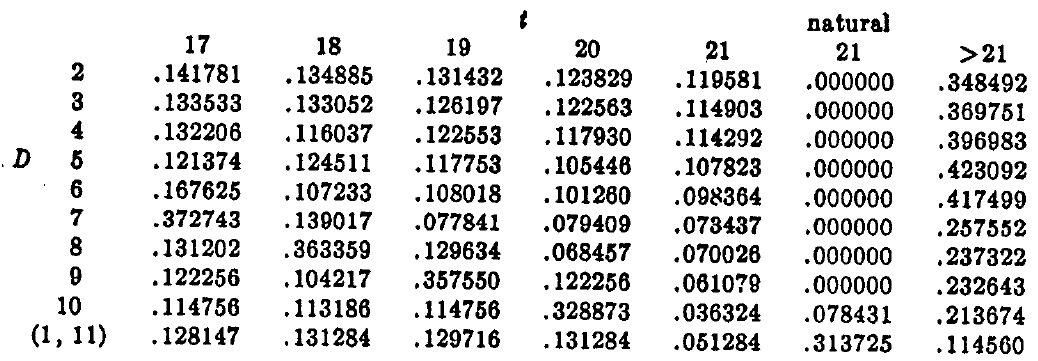
\includegraphics[width=0.8\linewidth]{tabla_probabilidades_baldwin} 

}

\caption{\label{forma_extensiva}Diagrama Juego}\label{fig:ingles_blackjack}
\end{figure}

Podemos ver que los resultados son muy similares, por lo que podemos
deducir que los cálculos que hemos realizado son correctos. Una vez
conocidas las probabilidades, ya estamos en disposición de calcular
\(G_0(x,D)\) como detallábamos al comienzo, \(\forall \ x=4,\cdots\) y
\(\forall \  D=2,\cdots,10,(1,11)\). Una vez construyamos los
\(G_0(x,D)\) los utilizamos para implementarlos en el algoritmo,
teniendo en cuenta que si el máximo lo alcanzamos en dicho valor nos
plantaremos, y en caso contrario pediremos carta.

\begingroup\fontsize{12}{14}\selectfont

\begin{longtable}[t]{lcccccccccc}
\caption{\label{tab:unnamed-chunk-5}Tabla de procedimientos si el jugador posee una mano dura}\\
\toprule
 & 2 & 3 & 4 & 5 & 6 & 7 & 8 & 9 & Figura & As\\
\midrule
4 & C & C & C & C & C & C & C & C & C & C\\
5 & C & C & C & C & C & C & C & C & C & C\\
6 & C & C & C & C & C & C & C & C & C & C\\
7 & C & C & C & C & C & C & C & C & C & C\\
8 & C & C & C & C & C & C & C & C & C & C\\
\addlinespace
9 & C & C & C & C & C & C & C & C & C & C\\
10 & C & C & C & C & C & C & C & C & C & C\\
11 & C & C & C & C & C & C & C & C & C & C\\
12 & C & C & C & C & C & C & C & C & C & C\\
13 & C & P & P & P & P & C & C & C & C & C\\
\addlinespace
14 & P & P & P & P & P & C & C & C & C & C\\
15 & P & P & P & P & P & C & C & C & C & C\\
16 & P & P & P & P & P & C & C & C & C & C\\
17 & P & P & P & P & P & P & P & P & P & P\\
18 & P & P & P & P & P & P & P & P & P & P\\
\addlinespace
19 & P & P & P & P & P & P & P & P & P & P\\
20 & P & P & P & P & P & P & P & P & P & P\\
21 & P & P & P & P & P & P & P & P & P & P\\
22 & P & P & P & P & P & P & P & P & P & P\\
23 & P & P & P & P & P & P & P & P & P & P\\
\addlinespace
24 & P & P & P & P & P & P & P & P & P & P\\
25 & P & P & P & P & P & P & P & P & P & P\\
26 & P & P & P & P & P & P & P & P & P & P\\
27 & P & P & P & P & P & P & P & P & P & P\\
28 & P & P & P & P & P & P & P & P & P & P\\
\addlinespace
29 & P & P & P & P & P & P & P & P & P & P\\
30 & P & P & P & P & P & P & P & P & P & P\\
31 & P & P & P & P & P & P & P & P & P & P\\
\bottomrule
\end{longtable}
\endgroup{}

De esta forma ya tenemos calculado los topes que en el capitulo
\(\ref{Seccion3}\) denotamos como \(M(D)\):

\[
\begin{array}{cccccccccccc}
D & : & 2 & 3 & 4 & 5 & 6 & 7 & 8 & 9 & \text{Figura} & \text{As} \\
\hline
M(D) & : & 14 & 13 & 13 & 13 & 13 & 17 & 17 & 17 & 17 & 17
\end{array}
\]

\hypertarget{Seccion42}{%
\section{Manos blandas}\label{Seccion42}}

Ahora, nuestro propósito es hacer lo mismo para el caso de que el
jugador posea una mano blanda. La principal modificación reside en lo
que comentamos al comienzo, que si nos pasamos de 21 con este tipo de
manos recurrimos a contar ese As como un 1. Ahora llamamos
\(\bar G^*(x,b)\) a la ganancia esperada en el caso de manos blandas.

\[
\bar G^*(x,D) = Max \\ \{G_0(x,D), \sum_{c=1}^{10}P_c \bar G^*(x+c,D) \}
\] Como vemos la ecuación es exactamente igual al caso de manos duras.
Lo que diferencia el tratamiento son los valores finales que le damos a
\(\bar G^*(x,b)\), por el tratamiento diferente que reciben estas manos.
los valores iniciales son: \(\bar G^*(x,b) = G^*(x-10,D),x>21\) y
\(\forall D\)

Ahora nuestra regla de parada es la siguiente:

\begingroup\fontsize{12}{14}\selectfont

\begin{longtable}[t]{lcccccccccc}
\caption{\label{tab:unnamed-chunk-7}Tabla de procedimientos si el jugador posee una mano blanda}\\
\toprule
 & 2 & 3 & 4 & 5 & 6 & 7 & 8 & 9 & Figura & As\\
\midrule
4 & C & C & C & C & C & C & C & C & C & C\\
5 & C & C & C & C & C & C & C & C & C & C\\
6 & C & C & C & C & C & C & C & C & C & C\\
7 & C & C & C & C & C & C & C & C & C & C\\
8 & C & C & C & C & C & C & C & C & C & C\\
\addlinespace
9 & C & C & C & C & C & C & C & C & C & C\\
10 & C & C & C & C & C & C & C & C & C & C\\
11 & C & C & C & C & C & C & C & C & C & C\\
12 & C & C & C & C & C & C & C & C & C & C\\
13 & C & C & C & C & C & C & C & C & C & C\\
\addlinespace
14 & C & C & C & C & C & C & C & C & C & C\\
15 & C & C & C & C & C & C & C & C & C & C\\
16 & C & C & C & C & C & C & C & C & C & C\\
17 & C & C & C & C & C & C & C & C & C & C\\
18 & C & C & P & P & P & P & C & C & C & C\\
\addlinespace
19 & P & P & P & P & P & P & P & P & C & C\\
20 & P & P & P & P & P & P & P & P & P & P\\
21 & P & P & P & P & P & P & P & P & P & P\\
22 & P & P & P & P & P & P & P & P & P & P\\
23 & P & P & P & P & P & P & P & P & P & P\\
\addlinespace
24 & P & P & P & P & P & P & P & P & P & P\\
25 & P & P & P & P & P & P & P & P & P & P\\
26 & P & P & P & P & P & P & P & P & P & P\\
27 & P & P & P & P & P & P & P & P & P & P\\
28 & P & P & P & P & P & P & P & P & P & P\\
\addlinespace
29 & P & P & P & P & P & P & P & P & P & P\\
30 & P & P & P & P & P & P & P & P & P & P\\
31 & P & P & P & P & P & P & P & P & P & P\\
\bottomrule
\end{longtable}
\endgroup{}

Y ya tenemos calculados los topes que llamamos \(M^*(D)\):

\[
\begin{array}{cccccccccccc}
D & : & 2 & 3 & 4 & 5 & 6 & 7 & 8 & 9 & \text{Figura} & \text{As} \\
\hline
M^*(D) & : & 19 & 19 & 18 & 18 & 18 & 18 & 19 & 19 & 20 & 20
\end{array}
\]

\hypertarget{Seccion43}{%
\section{Doblar la apuesta}\label{Seccion43}}

Para poder doblarnos los valores de las dos primeras cartas deben sumar
9, 10 u 11, recibiendo una carta mas y solo una si lo hace. Así tenemos
las siguientes situaciones \((9,D)\), \((10,D)\), \((11,D)\),
\(\forall D\). Ahora tenemos que calcular la ganancia esperada de doblar
nuestra apuesta, en función de la carta que nos toque y compararla con
la ganancia esperada en el caso de no hacerlo, resultando en:

\[
\begin{array}{cllll}
\text{Si} & 2 \sum_{c=1}^{10}P_cG_0(x+c,b) & > & G^*(x,b) & \text{doblar apuesta} \\
\text{Si} & 2 \sum_{c=1}^{10}P_cG_0(x+c,b) & \leq & G^*(x,b) & \text{no doblar apuesta}\\
\end{array}
\]

Y la estrategia optima de cuando doblarse y cuando no es la siguiente:

\begingroup\fontsize{12}{14}\selectfont

\begin{longtable}[t]{lcccccccccc}
\caption{\label{tab:unnamed-chunk-9}Tabla de procedimientos para decidir si doblarse o no}\\
\toprule
 & 2 & 3 & 4 & 5 & 6 & 7 & 8 & 9 & Figura & As\\
\midrule
9 & No D & D & D & D & D & No D & No D & No D & No D & No D\\
10 & D & D & D & D & D & D & D & D & No D & No D\\
11 & No D & No D & No D & No D & D & No D & No D & No D & No D & No D\\
\bottomrule
\end{longtable}
\endgroup{}

\hypertarget{Seccion44}{%
\section{Abrise y jugar a dos manos}\label{Seccion44}}

En este apartado tendremos que comparar la ganancia esperada cuando no
nos abrimos y jugamos de manera óptima como hicimos en los subapartados
\(\ref{Seccion41}\) y \(\ref{Seccion41}\), a la ganancia que tendríamos
en el caso de abrirnos y jugar óptimamente cada una de las manos.

Así, construimos la siguiente regla que nos marca que camino tenemos que
coger:

\[
\begin{array}{cllll}
\text{Si} & 2 \sum_{c=1}^{10}P_cG^*(z+c,b) & > & G^*(2z,b) & \text{Abrirse} \\
\text{Si} & 2 \sum_{c=1}^{10}P_cG^*(z+c,b) & \leq & G^*(2z,b) & \text{No abrirse}\\
\end{array}
\] Donde \(z\) es la carta que recibimos doble. Aquí nos encontramos un
pequeño impedimento que es el caso cuando recibimos dos Ases, en este
caso tendríamos que:

\[
\begin{array}{cllll}
\text{Si} & 2 \sum_{c=1}^{10}P_cG_0(11+c,b) & > & \bar G^*(12,b) & \text{Abrirse} \\
\text{Si} & 2 \sum_{c=1}^{10}P_cG_0(11+c,b) & \leq & \bar G^*(12,b)& \text{No abrirse}\\
\end{array}
\]

Y obtendríamos las siguiente tabla con los procedimientos que debe
llevar el jugador:

\begingroup\fontsize{12}{14}\selectfont

\begin{longtable}[t]{lcccccccccc}
\caption{\label{tab:unnamed-chunk-11}Tabla de procedimientos para decidir si abrirse o no}\\
\toprule
 & 2 & 3 & 4 & 5 & 6 & 7 & 8 & 9 & Figura & As\\
\midrule
2-2 & No A & No A & A & A & A & A & No A & No A & No A & No A\\
3-3 & No A & No A & No A & A & A & A & No A & No A & No A & No A\\
4-4 & No A & No A & No A & No A & No A & No A & No A & No A & No A & No A\\
5-5 & No A & No A & No A & No A & No A & No A & No A & No A & No A & No A\\
6-6 & No A & A & A & A & A & No A & No A & No A & No A & No A\\
\addlinespace
7-7 & A & A & A & A & A & A & No A & No A & No A & No A\\
8-8 & A & A & A & A & A & A & A & A & No A & No A\\
9-9 & A & A & A & A & A & A & A & A & No A & No A\\
Figura-Figura & No A & No A & No A & No A & No A & No A & No A & No A & No A & No A\\
As-As & No A & A & A & A & A & No A & No A & No A & No A & No A\\
\bottomrule
\end{longtable}
\endgroup{}

\hypertarget{Seccion45}{%
\section{Asegurarse}\label{Seccion45}}

Suponemos ahora que la carta visible del crupier es un As. La apuesta
adicional que puede hacer el jugador es de un valor \(v\),
\(v \leq \frac{1}{2}\). Lo que ocurre aquí, es que el jugador decide
asegurarse, su mano ya no compite contra el crupier, sino que el compite
contra el hecho de que el crupier obtenga un BlacjJack. Por ejemplo, si
la suma de cartas del jugador es 13 y la primera carta del crupier es un
As, este podría asegurarse. En caso de hacerlo, si el crupier no
obtuviera BlackJack, obtuviera una suma de 20, el jugador gana aunque su
suma es inferior a la suma del crupier.

Esta apuesta por tanto se reduce al hecho de que salga una figura o no.
La probabilidad de que salga una figura, como desde un comienzo estamos
en la hipótesis de sucesos equiprobables, es de \(\frac{16}{52}\) que es
aproximadamente \(0.3077 \rightarrow 30,77 \%\). Llamemosle \(p\) a la
probabilidad de que salga una figura, obteniendo el crupier un
blackjack. Supongamos que la cantidad con la que nos aseguramos es
\(v=\frac{1}{2}\). Entonces nos interesa que el valor esperado al
asegurarnos sea no negativo al menos.

El valor esperado lo podemos calcular con la fórmula
\(E[ \ Asegurarse \ ]= 1·p - \frac{1}{2}·(1-p)\) veamos cuando esa
esperanza es mayor o igual a 0:

\[
\begin{array}{ccl}
p - \frac{1}{2}(1-p)& \geq  & 0 \\
p - \frac{1}{2} +\frac{1}{2}p& \geq  & 0\\
\frac{3}{2}p - \frac{1}{2} & \geq  & 0\\
3p - 1& \geq  & 0 \\
p & \geq & \frac{1}{3}
\end{array}
\] Es decir, para que asegurarse sea rentable la probabilidad debe ser
al menos de un tercio, \(33,3 \%\), por lo que no sería rentable
asegurarse, ya que la probabilidad que tenemos actualmente es inferior.
Esta probabilidad podría aumentar si el jugador viese si faltan muchas
figuras por salir de la baraja.

Como hemos asumido como hipótesis inicial que sacar una carta es
equiprobable a sacar otra, es decir, no contamos cartas, descartamos el
hecho de que asegurarse sea rentable a la larga y por lo tanto la
conclusión es no asegurarse.

Algo que podemos hacer es construir la forma normal del juego para ver
como sería este reparto:

\begingroup\fontsize{12}{14}\selectfont

\begin{longtable}[t]{lcc}
\caption{\label{tab:unnamed-chunk-12}Forma normal cuando jugador posee un Blackjack}\\
\toprule
 & C BJ & C No BJ\\
\midrule
J Asegura & 1 & 1.0\\
J No Asegura & 0 & 1.5\\
\bottomrule
\end{longtable}
\endgroup{}

Esto podríamos extenderlo a todos los casos, cuando la suma del jugador
es \(x\), que no es un Blackjack, y en caso de no conseguir un
Blackjack, la suma del crupier es \(T\) a lo siguiente y calcular las
ganancias esperadas en cada caso en función de la probabilidades de que
\(T\) supere a \(x\) o no

\hypertarget{Seccion46}{%
\section{Conclusion. Utilidad de seguir la estrategia
óptima.}\label{Seccion46}}

Ahora ya tenemos determinada nuestra estrategia optima, en la que
sabemos en que suma de cartas debemos plantando en función de si tenemos
una mano dura o una mano blanda; si debemos doblarnos o no dependiendo
de la carta que tenga visible el crupier; si debemos abrirnos y jugar a
dos manos siguiendo las estrategias anteriormente comentadas; y si
debemos asegurarnos, que sabemos que nunca lo debemos hacer.

Nuestro objetivo ahora es calcular cuantas unidades monetarias
obtendremos por cada una apostada en este juego, si siguiéramos la
estrategia ideal anteriormente expuesta. Nos apoyamos en \citep{Libro9}

Para ello, para cada situación inicial que se presenta, carta visible
del crupier mas las dos cartas iniciales del jugador se genera una
cantidad grande de jugadas calculando la cantidad media de ganancia
obtenida en cada una mediante los métodos de montecarlo y se pondera por
la probabilidad de que suceda esa mano. Hemos utilizado 100 muestras
generando el siguiente gráfico:

\begin{figure}[H]

{\centering \includegraphics[width=0.95\linewidth]{figurasR/unnamed-chunk-14-1} 

}

\caption{Gráfica de la esperanza del Blackjack \label{esperanza_blackjack}}\label{fig:unnamed-chunk-14}
\end{figure}

Nos damos cuenta que todas las esperanzas que se calculan en cada una de
las muestras es negativa. Pasamos ahora a calcular la media y un
intervalo de confianza al \(95 \%\). Así obtenemos los siguientes datos:

\begin{enumerate}
\def\labelenumi{\arabic{enumi}.}
\item
  Valor esperado del juego: -0.19401
\item
  Límite inferior del intervalo de confianza: -0.1958367
\item
  Límite superior del intervalo de confianza: -0.1921833
\end{enumerate}

De aquí podemos deducir que el limite superior del intervalo siempre es
negativo por lo que la conclusión final es que perderíamos parte del
dinero apostado (en torno al \(20 \%\)), aun jugando la estrategia
óptima, y por tanto no merece la pena intentar jugar al Blackjack para
intentar ganar dinero, pues el crupier y por tanto el casino ganan.

\bibliography{bib/library.bib,bib/paquetes.bib}


%


\end{document}
